\chapter{Наборы данных и функции потерь}
\label{chap:supervised_learning}

\begin{supportbox}{Об этой главе}
В этой главе формализуется сценарий обучения с учителем. Мы вводим понятия наборов данных, функций потерь и минимизации эмпирического риска, подчеркивая основные допущения, сделанные в обучении с учителем. В заключение мы приводим вероятностную формулировку обучения с учителем, основанную на понятии максимального правдоподобия. Эта короткая глава служит основой для остальной части книги.
\end{supportbox}

\section{Что такое набор данных?}
\label{sec:dataset}

Мы рассматриваем сценарий, в котором ручное кодирование определенной функции нецелесообразно (например, распознавание объектов на реальных изображениях), но сбор \textbf{примеров} желаемого поведения достаточно прост. Примеров этого предостаточно, от распознавания речи до навигации роботов. Мы формализуем эту идею следующим определением.

\begin{definition}[Набор данных] \addbottle
\textbf{Набор данных для обучения с учителем} $\mathcal{S}_n$ размера $n$ — это множество из $n$ пар $\mathcal{S}_n = \left\{(x_i, y_i)\right\}_{i=1}^n$, где каждая пара $(x_i, y_i)$ является примером вход-выходной зависимости, которую мы хотим смоделировать. Мы также предполагаем, что каждый пример является \textbf{одинаково} и \textbf{независимо} распределенной (i.i.d.) выборкой из некоторого неизвестного (и непознаваемого) распределения вероятностей $p(x,y)$.
\end{definition}

См. Приложение \ref{chap:probability_theory}, если после прочтения определения вы захотите освежить свои знания по теории вероятностей. Последнее предположение кажется техническим, но оно необходимо для того, чтобы гарантировать, что моделируемая нами зависимость имеет смысл. В частности, то, что выборки \textbf{одинаково распределены}, означает, что мы пытаемся аппроксимировать нечто достаточно стабильное и неизменное во времени. В качестве характерного примера рассмотрим задачу сбора набора данных для распознавания моделей автомобилей по фотографиям. Это предположение будет выполнено, если мы будем собирать изображения в течение короткого промежутка времени, но оно будет неверным, если собирать изображения за последние несколько десятилетий, поскольку модели автомобилей со временем изменились. В последнем случае обучение и развертывание модели на этом наборе данных потерпят неудачу, поскольку она не сможет распознавать новые модели или будет иметь неоптимальную производительность при использовании.

Аналогично, то, что выборки \textbf{независимо распределены}, означает, что в нашем наборе данных нет смещения при сборе, и он достаточно репрезентативен для всего распределения. Возвращаясь к предыдущему примеру, сбор изображений рядом с дилерским центром Tesla будет неверным, поскольку мы соберем избыток изображений определенного типа, упустив изображения других производителей и моделей. Обратите внимание, что справедливость этих предположений зависит от контекста: набор данных автомобилей, собранный в Италии, может быть действителен при развертывании нашей модели в Риме или Милане, но может быть недействителен при развертывании нашей модели в Токио или на Тайване. Предположение i.i.d. всегда следует тщательно проверять, чтобы убедиться, что мы применяем наши инструменты обучения с учителем к действительному сценарию. Интересно, что современные БЯМ обучаются на таких больших распределениях данных, что даже понимание того, какие задачи действительно находятся \textit{в распределении}, а какие \textit{вне распределения} (и насколько модели способны к обобщению), становится размытым \cite{yuan2024revisiting}.

\subsection{Варианты обучения с учителем}
\label{subsec:variants_supervised_learning}

\begin{figure}[t]
    \centering
    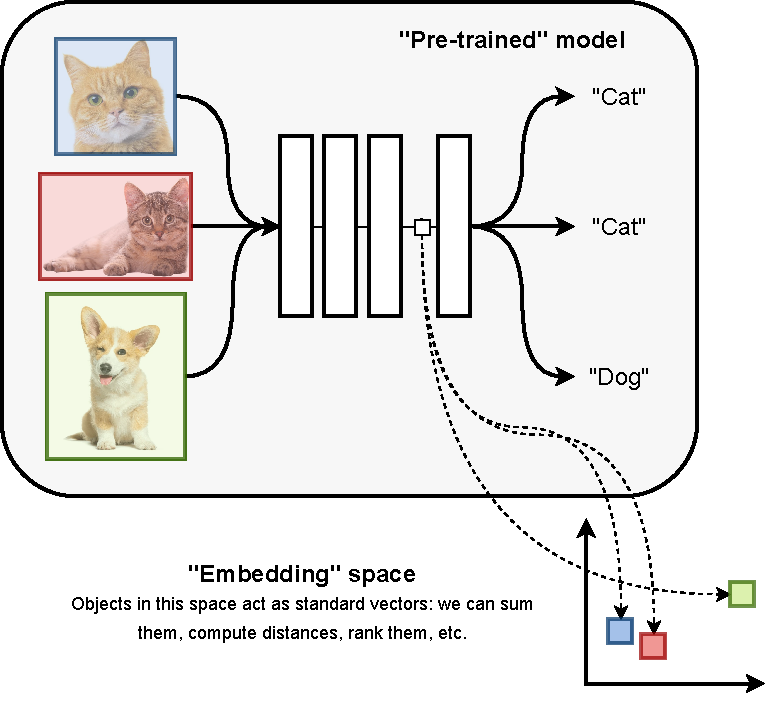
\includegraphics[width=0.7\textwidth]{images/embedding.pdf}
    \caption{Дифференцируемые модели обрабатывают данные, последовательно преобразуя их с помощью операций линейной алгебры. Во многих случаях после оптимизации этих программ внутренние представления входных данных модели (то, что мы называем \textbf{предварительно обученной} моделью) имеют геометрические свойства: например, семантически схожие изображения проецируются в точки, которые близки в этом «скрытом» пространстве. Преобразование данных из неметрического пространства (исходные входные изображения) в метрическое пространство (внизу справа) называется \textbf{вложением} данных.}
    \label{fig:embedding}
\end{figure}

Существует множество вариаций стандартного сценария обучения с учителем, хотя большинство успешных приложений в той или иной форме используют обучение с учителем. Например, в некоторых наборах данных могут отсутствовать \textbf{целевые значения} $y_i$, и в этом случае мы говорим об \textbf{обучении без учителя}. Типичными приложениями обучения без учителя являются алгоритмы \textbf{кластеризации}, в которых мы хотим сгруппировать наши входные данные в \textit{кластеры} так, чтобы точки в одном кластере были похожи, а точки между кластерами — непохожи \cite{hastie2009elements}. В качестве другого примера, в системе \textbf{поиска} мы можем захотеть найти в большой базе данных $k$ наиболее похожих элементов на запрос пользователя.

При работе со сложными данными, такими как изображения, это нетривиально, потому что расстояния на изображениях плохо определены, если мы работаем с пикселями (т.е. даже небольшие возмущения могут изменить миллионы пикселей). Однако предположим, что у нас есть некоторая (дифференцируемая) модель, которую мы уже оптимизировали для какой-то другой, достаточно общей задачи, например, классификации изображений. Мы называем ее \textbf{предварительно обученной} моделью. Как мы увидим, внутренние состояния этой модели можно интерпретировать как векторы в многомерном пространстве. Во многих случаях эти векторы демонстрируют полезные геометрические свойства, в том смысле, что семантически схожие объекты отображаются (\textbf{вкладываются}) в точки, которые близки в этих представлениях. Следовательно, мы можем использовать эти скрытые представления со стандартными моделями кластеризации, такими как модели гауссовых смесей \cite{huang2014deep}. См. Рисунок \ref{fig:embedding} для общего обзора этой идеи.

Что, если у нас нет доступа к предварительно обученной модели? Распространенный вариант обучения без учителя называется \textbf{самообучением} (SSL, \cite{zbontar2021barlow}). Цель SSL — автоматически найти некоторую задачу обучения с учителем из общего набора данных без учителя, чтобы оптимизировать модель, которую можно будет использовать в большом наборе последующих задач. Например, если у нас есть доступ к большому корпусу текста, мы всегда можем оптимизировать программу для предсказания вероятного продолжения небольшого фрагмента текста \cite{radford2019language}. Осознание того, что нейронные сети также могут выполнять эффективное вложение текста при предварительном обучении в режиме самообучения, оказало глубокое влияние на сообщество \cite{mikolov2013distributed}.\footnote{Крупномасштабные веб-наборы данных также полны предвзятости, ненормативной лексики и вульгарного контента. Признание того, что модели, обученные на этих данных, усваивают эти предвзятости, было еще одним важным осознанием \cite{bolukbasi2016man} и является одной из основных критик моделей-оснований с закрытым исходным кодом \cite{bender2021dangers}.}

\begin{figure}[t]
    \centering
    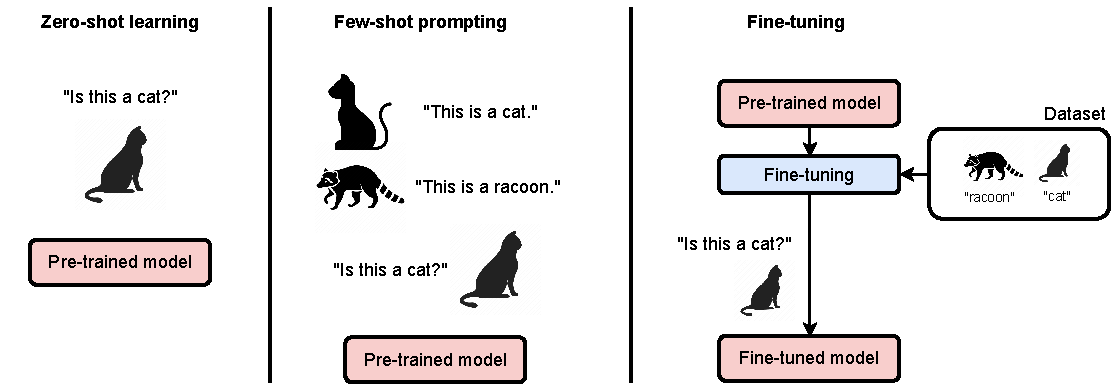
\includegraphics[width=0.95\textwidth]{images/using_models.pdf}
    \caption{Три способа использования обученных моделей. \textbf{Нулевой выстрел}: вопрос напрямую задается модели. Этого можно достичь с помощью генеративных языковых моделей (представленных в Главе \ref{chap:convolutions_beyond_images}). \textbf{Промптинг с несколькими примерами} похож, но в качестве входных данных предоставляется несколько примеров. Обе техники могут применяться только в том случае, если базовая модель демонстрирует большие возможности обобщения. \textbf{Дообучение}: модель оптимизируется с помощью градиентного спуска на небольшом наборе данных примеров. Это происходит аналогично обучению модели с нуля.}
    \label{fig:using_models}
\end{figure}

Как мы увидим в Главе \ref{chap:convolutions_beyond_images} и Главе \ref{chap:transformers}, БЯМ можно рассматривать как современные итерации этой основной идеи, поскольку оптимизация моделей, таких как GPT или Llama \cite{touvron2023llama}, всегда начинается с базового самообучения в терминах предсказания следующего токена. Эти модели иногда называют \textbf{фундаментальными моделями}. В простейшем случае их можно использовать «из коробки» для новой задачи, например, для ответа на запрос: в этом случае мы говорим, что они используются в режиме \textbf{нулевого выстрела}. Для БЯМ также возможно предоставить небольшое количество примеров новой задачи в качестве входного промпта, и в этом случае мы говорим о \textbf{промптинге с несколькими примерами}. В самом общем случае мы можем взять предварительно обученную фундаментальную модель и оптимизировать ее параметры с помощью градиентного спуска для новой задачи: это называется \textbf{дообучением} модели. См. Рисунок \ref{fig:using_models} для сравнения трех подходов. В этой книге мы сосредоточимся на создании моделей с нуля, но дообучение можно проводить аналогичными способами.

Дообучение особенно упрощается благодаря наличию больших репозиториев с открытым исходным кодом в Интернете.\footnote{\url{https://huggingface.co/models}} Дообучение можно проводить на полном наборе параметров исходной модели или, рассматривая только меньшее подмножество или небольшое количество дополнительных параметров: это называется \textbf{параметрически-эффективным дообучением} (PEFT) \cite{lialin2023scaling}.\footnote{Обучение с несколькими примерами также можно проводить путем дообучения модели. В случаях, когда дообучение не требуется, мы говорим, что модель выполняет \textbf{обучение в контексте} \cite{akyurek2022learning}.}

Возможны многие другие вариации обучения с учителем, которые мы не можем подробно перечислить здесь, за исключением некоторых общих намеков. Если помечена только часть набора данных, у нас есть \textbf{полууправляемый} сценарий \cite{belkin2006manifold}. Мы увидим некоторые примеры полууправляемого обучения в Главе \ref{chap:gnns}. Кроме того, у нас могут быть сценарии с несколькими наборами данных, принадлежащими к «похожим» распределениям, или одному и тому же распределению в разные периоды времени, что порождает бесчисленные задачи в зависимости от порядка, в котором предоставляются задачи или данные, включая \textbf{адаптацию домена}, \textbf{мета-обучение} \cite{finn2017model}, \textbf{непрерывное обучение} \cite{parisi2019continual,biesialska2020continual}, \textbf{метрическое обучение}, \textbf{разучивание} и т.д. Некоторые из них будут рассмотрены в следующем томе.

\begin{supportbox}{Подробнее о свойстве i.i.d.}
Важно отметить, что обеспечение свойства i.i.d. — это не одноразовый процесс, и его необходимо постоянно проверять в течение всего срока службы модели. В случае классификации автомобилей, если это не проверять, тонкие изменения в распределении автомобилей со временем приведут к ухудшению производительности модели машинного обучения, что является примером \textbf{сдвига домена}. В качестве другого примера, рекомендательная система изменит способ взаимодействия пользователей с определенным приложением, поскольку они начнут реагировать на предложения самой рекомендательной системы. Это создает \textbf{петли обратной связи} \cite{cinus2022effect}, которые требуют постоянной переоценки производительности системы и приложения.
\end{supportbox}

\section{Функции потерь}
\label{sec:loss_functions}

\addclock После сбора данных нам необходимо формализовать нашу идею «аппроксимации» желаемого поведения, что мы делаем, вводя понятие \textbf{функций потерь}.

\begin{definition}[Функция потерь] \addbottle
Для желаемой цели $y$ и предсказанного значения $\hat{y}=f(x)$ из модели $f$, \textbf{функция потерь} $l(y, \hat{y}) \in \mathbb{R}$ — это скалярная, дифференцируемая функция, значение которой коррелирует с производительностью модели, т.е. $l(y, \hat{y}_1) < l(y, \hat{y}_2)$ означает, что предсказание $\hat{y}_1$ лучше, чем предсказание $\hat{y}_2$, при рассмотрении эталонного значения (цели) $y$.
\end{definition}

Функция потерь воплощает наше понимание задачи и наши предпочтения в пространстве решений в виде вещественной шкалы, которую можно использовать в алгоритме оптимизации. Будучи дифференцируемой, она позволяет нам превратить нашу задачу обучения в задачу математической оптимизации, которую можно решить с помощью градиентного спуска, минимизируя средние потери на нашем наборе данных.

Для этого, имея набор данных $\mathcal{S}_n = \left\{(x_i, y_i)\right\}$ и функцию потерь $l(\cdot, \cdot)$, разумной задачей оптимизации является минимизация средней потери на наборе данных, достижимая любой возможной \textit{дифференцируемой} моделью $f$:

\vspace{1em}
\begin{equation}
    f^* = \underset{f}{\arg\min} \;\; \eqnmarkbox[drawred]{node}{\frac{1}{n}\sum_{i=1}^n} l(y_i, \eqnmarkbox[drawblue]{node2}{f(x_i)})
    \label{eq:empirical_risk_minimization}
\end{equation}
\annotate[yshift=1em]{above,right}{node}{Среднее по набору данных}
\annotate[yshift=-1.5em]{below,left}{node2}{Предсказание $f$ на $i$-м примере из набора данных}

\vspace{1em}
По историческим причинам \eqref{eq:empirical_risk_minimization} называется \textbf{минимизацией эмпирического риска} (ERM), где \textit{риск} используется как общий синоним \textit{потерь}. См. также вставку на следующей странице для получения дополнительной информации о происхождении термина.

В \eqref{eq:empirical_risk_minimization} мы неявно предполагаем, что минимизируем по пространству всех возможных функций, определенных на нашем входе $x$. Вскоре мы увидим, что наши модели всегда можно параметризовать набором тензоров $w$ (называемых \textbf{параметрами} модели), и минимизация выполняется путем поиска оптимального значения этих параметров с помощью численной оптимизации, которую мы обозначаем как $f(x,w)$. Следовательно, имея набор данных $\mathcal{S}_n$, функцию потерь $l$ и пространство моделей $f$, мы можем \textbf{обучать} нашу модель, оптимизируя эмпирический риск \eqref{eq:empirical_risk_minimization} с помощью градиентного спуска \eqref{eq:gradient_descent}:
%
\begin{equation}
    {\color{drawred}w^*} = \underset{w}{\arg\min} \;\; \frac{1}{n}\sum_{i=1}^n l(y_i, f(x_i, {\color{drawred}w}))
    \label{eq:empirical_risk_minimization_2}
\end{equation}
%
где минимизация теперь выполняется по отношению к тензору параметров $w$.

\subsection*{О дифференцируемости потерь}
\label{subsec:differentiability_loss}

 Прежде чем продолжить, сделаем два замечания о фреймворке ERM. \addteacup Во-первых, обратите внимание, что требование дифференцируемости $l$ является фундаментальным. Рассмотрим простую задачу \textbf{бинарной классификации} (которую мы должным образом представим в следующей главе), где $y \in \left\{-1,+1\right\}$ может принимать только два значения, $-1$ или $1$. Для вещественнозначной модели $f(x) \in \mathbb{R}$ мы можем приравнять два решения к знаку $f$ — который мы обозначаем как $\text{sign}(f(x))$ — и определить \textbf{потери 0/1} как:
%
\begin{equation}
l(y, \hat{y})=\begin{cases} 0 & \text{ если } \text{sign}(\hat{y}) = y \\ 1 & \text{ иначе } \end{cases}
\label{eq:01_loss}
\end{equation}
%
Хотя это соответствует нашему интуитивному представлению о «правоте», это бесполезно в качестве функции потерь, поскольку ее градиент почти всегда будет равен нулю (за исключением случаев, когда знак $f$ меняется), и любой алгоритм градиентного спуска застрянет на инициализации. Менее интуитивной величиной в этом случае является \textbf{отступ} $y\hat{y}$, который положителен [отрицателен] в зависимости от того, совпадает ли знак модели с желаемым [или не совпадает], но он изменяется непрерывно, в отличие от потерь 0/1 в \eqref{eq:01_loss}. 

Возможной функцией потерь в этом случае является \textbf{шарнирная функция потерь} $l(y,\hat{y}) = \max(0, 1 - y\hat{y})$, которая используется для обучения моделей опорных векторов. Детали в стороне, это показывает внутреннее напряжение между разработкой функций потерь, которые кодируют наше представление о производительности, и в то же время являются полезными для численной оптимизации.

\subsection{Ожидаемый риск и переобучение}

Во-вторых, обратите внимание, что эмпирический риск всегда тривиально минимизировать, определив:

\begin{equation}
f(x) = \begin{cases} y & \text{ если } \eqnmarkbox[drawred]{node}{(x,y) \in \mathcal{S}_n} \\ \eqnmarkbox[drawblue]{node2}{\bar{y}} & \text{ иначе} \end{cases} \;.
\label{eq:lookup_table}
\end{equation}
\annotate[yshift=1em]{above,right}{node}{$x$ находится в обучающем наборе}
\annotate[yshift=-1em]{below,right}{node2}{Значение по умолчанию, например, $0$}

\vspace{1em}
Это таблица поиска, которая возвращает предсказание $y$, если пара $(x,y)$ содержится в наборе данных, а в противном случае возвращает некоторое постоянное предсказание $\bar{y}$ (например, 0). Предполагая, что потери ограничены снизу, когда $y = \hat{y}$, эта модель всегда будет достигать наименьшего возможного значения эмпирического риска, не имея при этом никакой практической ценности. 

Это показывает разницу между \textbf{запоминанием} и \textbf{обучением} (оптимизацией). Хотя мы ищем модель, оптимизируя некоторую среднюю величину потерь на наших обучающих данных, как в \eqref{eq:empirical_risk_minimization}, нашей истинной целью является минимизация этой величины на некотором неизвестном, будущем входе, который еще предстоит увидеть. Элементы нашего обучающего набора являются лишь средством для достижения этой цели. Мы можем формализовать эту идею, определив задачу \textbf{минимизации ожидаемого риска}.

\begin{definition}[Ожидаемый риск]
Для распределения вероятностей $p(x,y)$ и функции потерь $l$, \textbf{ожидаемый риск} (ER) определяется как:
%
\begin{equation}
\textnormal{ER}[f] = \mathbb{E}_{p(x,y)}\left[ l(y, f(x)) \right]
\label{eq:expected_risk}
\end{equation}
\end{definition}

Минимизацию \eqref{eq:expected_risk} можно интерпретировать как минимизацию средней (ожидаемой) потери по \textit{всем возможным парам вход-выход} (например, всем возможным электронным письмам), которые может увидеть наша модель. Очевидно, что модель с низким ожидаемым риском гарантированно будет работать правильно. Однако величина в \eqref{eq:expected_risk} на практике невычислима, так как перечисление и маркировка всех точек данных невозможны. Эмпирический риск дает оценку ожидаемого риска при выборе данного набора данных и может рассматриваться как аппроксимация методом Монте-Карло члена ER.

Разница в потерях между ожидаемым и эмпирическим риском называется \textbf{разрывом обобщения}: алгоритм чистого запоминания, подобный \eqref{eq:lookup_table}, будет иметь плохую обобщающую способность или, другими словами, он будет \textbf{переобучаться} на конкретные предоставленные нами обучающие данные. Обобщение можно проверить на практике, оставив отдельный \textbf{тестовый набор данных} $\mathcal{T}_m$ с $m$ точками данных, никогда не использовавшимися во время обучения, $\mathcal{S}_n \cap \mathcal{T}_m = \emptyset$. Тогда разницу в эмпирических потерях между $\mathcal{S}_n$ и $\mathcal{T}_m$ можно использовать как приблизительную меру переобучения.

\begin{supportbox}{Риск и потери}
Минимизация эмпирического и ожидаемого риска, сформулированная таким образом, обычно ассоциируется с работами российского ученого В. Вапника \cite{vapnik2013nature}, которые положили начало области \textit{статистической теории обучения} (SLT). SLT особенно занимается поведением \eqref{eq:empirical_risk_minimization}, рассматриваемого как аппроксимация конечной выборкой \eqref{eq:expected_risk} при некотором ограниченном классе функций $f$ и мере базовой сложности \cite{poggio2003mathematics,shalev2014understanding,mohri2018foundations}. Контринтуитивные свойства современных нейронных сетей (такие как сильное обобщение далеко за пределами того, где следовало бы ожидать переобучения) открыли много новых направлений исследований в SLT \cite{poggio2020theoretical}. См. также введение к Главе \ref{chap:deep_cnns}.
\end{supportbox}

\subsection{Как выбрать правильную функцию потерь?} 
\label{subsec:how_to_select_a_loss}

\begin{tcolorbox}
Если вы еще этого не сделали, сейчас самое время изучить (или бегло просмотреть) материал в Приложении \ref{chap:probability_theory}, особенно распределения вероятностей, достаточные статистики и оценку максимального правдоподобия.
\end{tcolorbox}

Как мы увидим в следующих главах, функция потерь кодирует наши априорные знания о решаемой задаче и оказывает большое влияние на производительность. В некоторых случаях простых соображений о задаче достаточно для разработки правильных функций потерь (например, как это было сделано для шарнирной функции потерь в Разделе \ref{subsec:differentiability_loss}).

Однако можно работать более принципиально, переформулировав весь процесс обучения в чисто вероятностных терминах, как мы сейчас покажем. Эта формулировка предоставляет альтернативную точку зрения на обучение, которая может быть более интуитивной или более полезной в определенных сценариях. Это также предпочтительная точка зрения многих книг \cite{bishop2024deep}. Мы приводим основные идеи в этом разделе и рассмотрим конкретные приложения позже в книге.

Ключевое наблюдение заключается в следующем. В Разделе \ref{sec:dataset} мы начали с предположения, что наши примеры происходят из распределения $p(x, y)$. По правилу произведения вероятностей мы можем разложить $p(x,y)$ как $p(x,y) = p(x)p(y \mid x)$, так что $p(x)$ зависит от вероятности наблюдения каждого входа $x$, а условный член $p(y \mid x)$ описывает вероятность наблюдения определенного выхода $y$ при заданном входе $x$.\footnote{Мы также можем разложить его как $p(x, y) = p(x \mid y)p(y)$. Методы, требующие оценки $p(x)$ или $p(x \mid y)$, называются \textbf{генеративными}, в то время как методы, оценивающие $p(y \mid x)$, называются \textbf{дискриминативными}. За исключением языкового моделирования, в этой книге мы сосредоточимся на последнем случае. Мы рассмотрим генеративное моделирование более широко в следующем томе.} Аппроксимация $p(y \;\vert\; x)$ функцией $f(x)$ имеет смысл, если мы предполагаем, что масса вероятности в основном сосредоточена вокруг одной точки $y$, т.е. $p(y \;\vert\; x)$ близка к так называемой дельта-функции Дирака, и это значительно упрощает общую формулировку задачи.

Однако мы можем ослабить это предположение, предположив, что наша модель $f(x)$ не дает непосредственно предсказание, а используется вместо этого для параметризации достаточных статистик условного распределения вероятностей $p(y \mid f(x))$ по возможным выходам. Например, рассмотрим задачу классификации, где $y \in \left\{1,2,3\right\}$ может принимать три возможных значения. Мы можем предположить, что наша модель имеет три выхода, которые параметризуют категориальное распределение по этим классам, так что:
%
$$
p(\mathbf{y} \;\vert\; f(x)) = \prod_{i=1}^3 {f_i(x)}^{y_i}
$$
%
где $\mathbf{y} \sim \text{Binary}(3)$ — это one-hot кодирование класса $y$\footnote{Для целого числа $i$ его one-hot представление — это вектор из всех нулей, за исключением $i$-го элемента, который равен $1$. Это формально вводится в Разделе \ref{sec:linear_models_for_classification}.} и $f(x) \sim \Delta(3)$ — это предсказанные вероятности для каждого класса. В качестве другого примера, предположим, мы хотим предсказать одно скалярное значение $y \in \mathbb{R}$ (\textbf{регрессия}). Мы можем смоделировать это с помощью функции с двумя значениями $f(x) \sim (2)$ так, что предсказание является гауссианой с соответствующим средним и дисперсией:

\begin{equation}
p(y \;\vert\; f(x))=\mathcal{N}(y \mid f_1(x), \eqnmarkbox[drawred]{node}{f_2^2(x)})
\label{eq:gaussian_conditional_distribution}
\end{equation}
\annotate[yshift=-1em]{below,right}{node}{В квадрате для обеспечения положительности}

\vspace{1em}
где второй выход $f(x)$ возводится в квадрат, чтобы гарантировать, что предсказанная дисперсия остается положительной. Как видно, это очень общая схема, которая включает в себя наше предыдущее обсуждение и предоставляет больше гибкости разработчику, поскольку выбор конкретной параметризации для $p(y \;\vert\; x)$ может быть проще, чем выбор конкретной функции потерь $l(y, \hat{y})$. Кроме того, этот фреймворк предоставляет более непосредственный способ моделирования неопределенности, такой как дисперсия в \eqref{eq:gaussian_conditional_distribution}.
%
\subsection{Максимальное правдоподобие}
%
Как мы можем обучать вероятностную модель? Помните, что мы предположили, что выборки в нашем наборе данных $\mathcal{S}_n$ являются i.i.d. выборками из распределения вероятностей $p(x,y)$. Следовательно, для модели $f(x)$ вероятность, присвоенная самому набору данных конкретным выбором функции $f$, задается произведением вероятностей каждого примера в наборе данных:
%
$$
p(\mathcal{S}_n \;\vert\; f)=\prod_{i=1}^n p(y_i \;\vert\; f(x_i))
$$

Величина $p(\mathcal{S}_n \;\vert\; f)$ называется \textbf{правдоподобием} набора данных. При случайном выборе $f(x)$ модель будет присваивать вероятности более или менее случайным образом по всем возможным входам и выходам, и правдоподобие нашего конкретного набора данных будет небольшим. Разумной стратегией, таким образом, является выбор модели таким образом, чтобы правдоподобие набора данных было максимальным. Это прямое применение подхода максимального правдоподобия (см. Раздел \ref{sec:maximum_likelihood_estimation} в Приложении \ref{chap:probability_theory}).

\begin{definition}[Обучение с учителем как максимальное правдоподобие] \addbottle
Для набора данных $\mathcal{S}_n = \left\{(x_i, y_i)\right\}$ и семейства распределений вероятностей $p(y \;\vert\; f(x))$, параметризованных $f(x)$, решение по \textbf{максимальному правдоподобию} (МП) задается как:
%
$$
f^* = \underset{f}{\arg\max}\prod_{i=1}^n p(y_i \;\vert\; f(x_i)) \;.
$$
\end{definition}

Хотя мы снова остаемся с задачей оптимизации, теперь она следует непосредственно из законов вероятности после выбора всех распределений вероятностей, что контрастирует с предыдущим подходом, где конкретная функция потерь была частью пространства проектирования. Однако эти две точки зрения тесно связаны. Работая в логарифмическом пространстве и переходя к задаче минимизации, мы получаем:
%
$$
\underset{f}{\arg\max} \left\{ \log \prod_{i=1}^n p(y_i \;\vert\; f(x_i)) \right\} = \underset{f}{\arg\min} \left\{ \sum_{i=1}^n -\log(p(y_i \;\vert\; f(x_i))) \right\}
$$
%
Следовательно, две формулировки идентичны, если мы отождествим $-\log(p(y \;\vert\; f(x))$ с «псевдо-потерями», которые нужно оптимизировать. Как мы увидим, все функции потерь, используемые на практике, могут быть получены по принципу МП для конкретных выборов этого члена. Обе точки зрения интересны, и мы призываем читателей помнить о них по мере продвижения по книге.

\section{Еще больше вероятности: Байесовское обучение}
\label{sec:bayesian_learning}

\addteacup Здесь мы обсуждаем дальнейшее обобщение вероятностной формулировки, называемое \textbf{Байесовскими нейронными сетями} (БНС), которое представляет интерес в литературе. Мы приводим только общую идею и отсылаем читателя к одному из многих подробных руководств, например, \cite{jospin2022hands}, для получения более подробной информации.

Проектируя функцию вероятности $p(y \;\vert\; f(x))$ вместо непосредственно $f(x)$, мы можем обрабатывать ситуации, когда представляет интерес более одного предсказания (т.е. функция вероятности имеет более одной моды). Однако наша процедура все равно возвращает \textit{одну функцию} $f(x)$ из пространства всех возможных функций, в то время как может случиться, что действительна более чем одна параметризация во всем пространстве модели. В этом случае было бы полезно иметь доступ ко всем из них для более точного предсказания.

И снова, мы можем достичь этой цели, спроектировав еще одно распределение вероятностей, а затем позволив правилам вероятности вести нас. Поскольку мы теперь планируем получить распределение по всем возможным функциям, мы начинаем с определения \textbf{априорного распределения вероятностей} $p(f)$ по всем возможным функциям (еще раз напомним, что в остальной части книги $f$ будет описываться конечным набором параметров, и в этом случае априорное распределение $p(f)$ будет априорным распределением по этим весам). Например, мы увидим, что во многих ситуациях предпочтительны функции с меньшей нормой (поскольку они более стабильны), и в этом случае мы могли бы определить априорное распределение $p(f) \propto \frac{1}{\lVert f \rVert}$ для некоторой нормы $\lVert f \rVert$ функции $f$. 

После наблюдения набора данных вероятность $f$ смещается в зависимости от априорного распределения и правдоподобия, и обновление задается \textbf{теоремой Байеса}:

\vspace*{1em}
\begin{equation}
\eqnmarkbox[drawblue]{node2}{p(f \;\vert\; \mathcal{S}_n)}=\frac{p(\mathcal{S}_n \;\vert\; f)\eqnmarkbox[drawred]{node}{p(f)}}{p(\mathcal{S}_n)}
\label{eq:posterior_distribution}
\end{equation}
\annotate[yshift=1em]{above,left}{node}{Априорное (\textit{до} наблюдения набора данных)}
\annotate[yshift=-1em]{below,right}{node2}{Апостериорное (\textit{после} наблюдения набора данных)}

\vspace{1em}
Член $p(f \;\vert\; \mathcal{S}_n)$ называется \textbf{апостериорной функцией распределения}, в то время как член $p(\mathcal{S}_n)$ в знаменателе называется \textbf{свидетельством} и необходим для обеспечения правильной нормализации апостериорного распределения. Предположим пока, что у нас есть доступ к апостериорному распределению. В отличие от предыдущего случая, распределение может кодировать предпочтение более чем одной функции $f$, что может обеспечить лучшую предсказательную силу. Для входа $x$ мы можем сделать предсказание, усреднив все возможные модели на основе их апостериорного веса:

\vspace{1em}
\begin{equation}
p(y \;\vert\; x)=\int_f \eqnmarkbox[drawred]{node}{p(y \;\vert\; f(x))}\eqnmarkbox[drawblue]{node2}{p(f \;\vert\; \mathcal{S}_n)} \approx \eqnmarkbox[drawgreen]{node3}{\frac{1}{k}\sum_{i=1}^k} p(y \;\vert\; f_i(x))p(f_i \;\vert\; \mathcal{S}_n)
\label{predictive_distribution}
\end{equation}
\annotate[yshift=1em]{above,left}{node}{Предсказание $f(x)$}
\annotate[yshift=1.5em]{above,right}{node2}{Вес, присвоенный $f$}
\annotate[yshift=-1em]{below,right}{node3}{Аппроксимация методом Монте-Карло}

\vspace{1em}
где в правой части \eqref{predictive_distribution} мы аппроксимировали интеграл средним по методу Монте-Карло по $k$ случайным выборкам из апостериорного распределения $f_k \sim p(f \;\vert\; \mathcal{S}_n)$. Общая красота этой схемы омрачается тем фактом, что апостериорное распределение в общем случае невозможно вычислить в замкнутой форме, за исключением очень специфических выборов априорного распределения и правдоподобия \cite{bishop2006pattern}. В отсутствие этого приходится прибегать к приближенным решениям, либо с помощью \textbf{метода Монте-Карло по цепям Маркова}, либо с помощью \textbf{вариационного вывода} \cite{jospin2022hands}. Мы увидим в Разделе \ref{subsec:dropout} один пример байесовского подхода к параметрам модели, называемый \textbf{дропаутом Монте-Карло}.

Прежде чем закончить этот раздел, отметим два интересных факта об апостериорном распределении. Во-первых, предположим, что нас интересует только функция с наибольшей апостериорной плотностью. В этом случае член свидетельства можно проигнорировать, и решение разложить на два отдельных члена:

\begin{gather}
f^*=\underset{f}{\arg\max} \; p(\mathcal{S}_n \;\vert\; f)p(f) = \\
\underset{f}{\arg\max} \; \left\{\eqnmarkbox[drawred]{node}{\log p(\mathcal{S}_n \;\vert\; f)} + \eqnmarkbox[drawblue]{node2}{\log p(f)}\right\}
\end{gather}
\annotate[yshift=-1em]{below,left}{node}{Член правдоподобия}
\annotate[yshift=-1em]{below,right}{node2}{Член регуляризации}

Это называется решением по \textbf{максимуму апостериорной вероятности} (MAP). Если все функции имеют одинаковый априорный вес (т.е. $p(f)$ равномерно по пространству функций), то второй член является константой и задача сводится к решению по максимальному правдоподобию. Однако в общем случае решение MAP будет налагать штраф на функции, слишком сильно отклоняющиеся от нашего априорного распределения. Мы увидим, что это полезная идея для борьбы с переобучением и наложения определенных ограничений на функцию $f$. Член $\log p(f)$ обычно называется \textbf{регуляризатором} по пространству функций, поскольку он подталкивает решение к бассейну притяжения, определяемому априорным распределением.\footnote{Разница между решениями по максимальному правдоподобию и по максимуму апостериорной вероятности слабо связана с разницей между \textbf{частотной} и \textbf{байесовской} интерпретацией вероятности \cite{hackenberger2019bayes}, т.е. вероятности как частоты событий или вероятности как меры неопределенности. С очень общей точки зрения, МП рассматривает параметры как неизвестный фиксированный член, а данные — как случайную выборку, в то время как байесовский подход рассматривает данные как фиксированные, а параметры — как случайные переменные.} 

Во-вторых, полный байесовский подход предоставляет простой способ включения новых данных, например, нового набора данных $\mathcal{S}^\prime_n$ из того же распределения. Для этого мы заменяем априорную функцию в \eqref{eq:posterior_distribution} апостериорным распределением, которое мы вычислили на первой части набора данных, которое теперь представляет собой начальное предположение о возможных значениях $f$, которое обновляется при просмотре новых данных.\footnote{Думайте об исходной априорной функции как о распределении на $f$ после наблюдения начального \textit{пустого множества} значений.} Это может смягчить проблемы при онлайн-обучении моделей, в частности, так называемое \textit{катастрофическое забывание} старой информации \cite{kirkpatrick2017overcoming}.